\copyrightVincent

\beginDetail{20}

	\begin{saveblock}{comments}
		\begin{highlightblock}[linewidth=0.9\textwidth,gobble=8]
			% Make soul package work in beamer presentations
			% Source: https://tex.stackexchange.com/...
			\let\UL\ul
			\makeatletter
			\renewcommand\ul{
				\let\set@color\beamerorig@set@color
				\let\reset@color\beamerorig@reset@color
				\UL
			}
			...
		\end{highlightblock}
	\end{saveblock}

	\begin{frame}
		\frametitle{\lang,Comments,Comments,}

		\useblock{comments}
	\end{frame}

\endDetail

\begin{saveblock}{comments1}
	\begin{highlightblock}[linewidth=0.6\textwidth,gobble=8]
		% TODO Translate to English
		\section{Nonsense}

		Lorem ipsum dolor sit amet,
		\textfb{ornare} sit amet.

		\subsection{About $\sqrt{2}$}
	\end{highlightblock}
\end{saveblock}

\begin{saveblock}{comments2}
	\begin{highlightblock}[linewidth=0.6\textwidth,gobble=8]
		% TODO Translate to English
		\section{Nonsense}

		%Lorem ipsum dolor sit amet,
		%\textfb{ornare} sit amet.
		%
		%\subsection{About $\sqrt{2}$}
	\end{highlightblock}
\end{saveblock}

\begin{saveblock}{comments3}
	\begin{highlightblock}[linewidth=0.6\textwidth,gobble=8]
		% TODO Translate to English
		\section{Nonsense}

		Lorem ipsum dolor sit amet,
		\textfb{ornare} sit amet.
		
		%\subsection{About $\sqrt{2}$}
	\end{highlightblock}
\end{saveblock}

\begin{saveblock}{comments4}
	\begin{highlightblock}[linewidth=0.6\textwidth,gobble=8]
		% TODO Translate to English
		\section{Nonsense}

		Lorem ipsum dolor sit amet,
		\textbf{ornare} sit amet.
		
		\subsection{About $\sqrt{2}$}
	\end{highlightblock}
\end{saveblock}

\def\frameSelection{2}

\beginDetail{20}
	\def\frameSelection{1-}
\endDetail

\beginFrameWithSelection{\frameSelection}
	\frametitle{\lang,Comments,Comments,}

	\begin{columns}
		\begin{column}{0.6\textwidth}
			\unless\ifishandout
				\only<1>{\useblock{comments1}}
			\fi
			\only<2>{\useblock{comments2}}
			\unless\ifishandout
				\only<3>{\useblock{comments3}}
				\only<4>{\useblock{comments4}}
			\fi
		\end{column}
		\begin{column}{0.4\textwidth}
			\unless\ifishandout
				\only<1,3>{\textcolor{red}{Error! Undefined control sequence}}
			\fi
			\only<2>{\adjustbox{frame=1pt 5pt}{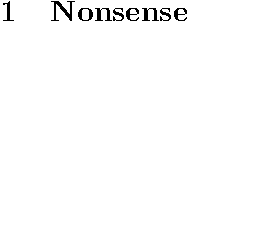
\includegraphics[
				width={\dimexpr\linewidth-12pt\relax},
				height=0.8\textheight,keepaspectratio]
			{assets/commentDebugSuccessEmptied.pdf}}}
			\unless\ifishandout\only<4>{\adjustbox{frame=1pt 5pt}{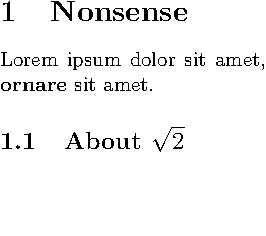
\includegraphics[
				width={\dimexpr\linewidth-12pt\relax},
				height=0.8\textheight,keepaspectratio]
			{assets/commentDebugSuccess.pdf}}}
			\fi
		\end{column}
	\end{columns}		
\end{frame}
